%%%%%%%%%%%%
%
% $Autor: Wings $
% $Datum: 2019-03-05 08:03:15Z $
% $Pfad: Automatisierung/Skript/Produktspezifikation/Powerpoint/AMF.tex $
% $Version: 4250 $
% !TeX spellcheck = en_GB/de_DE
% !TeX encoding = utf8
% !TeX root = filename 
% !TeX TXS-program:bibliography = txs:///biber
%
%%%%%%%%%%%%


\chapter{Computer Vision}

\section{Introduction}

Computer vision (CV) is an interdisciplinary scientific field that deals with how computers can gain high-level understanding from digital images or videos. It is the field of artificial intelligence (AI) that enables computers and systems to derive meaningful information from digital images, videos and other visual inputs — and take actions or make recommendations based on that information. \href{https://bit.ly/3iAQkv7}{Computer Vision} There is a lot of research being done in the computer vision field, but it’s not just research. Real-world applications demonstrate how important computer vision is to endeavors in business, entertainment, transportation, healthcare and everyday life. Scientists and engineers have been trying to develop ways for machines to see and understand visual data using Computer vision and Artificial Intelligence. Fig\ref{Computer Vision Chain} shows some of the application using computer vision.


\begin{figure}[h]
	\centering
	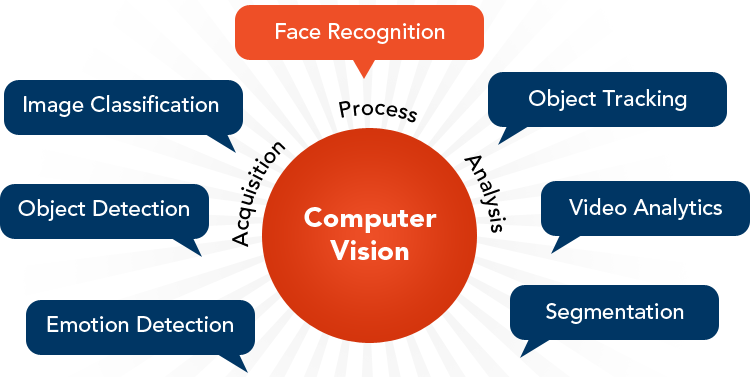
\includegraphics[width=0.7\linewidth]{Nano33BLESense/Computer Vision}
	\caption{Computer Vision Chain}
	\label{Computer Vision Chain}
\end{figure}

Computer Vision enables the computers to see, perceive and understand the world around them. This is achieved through a combination of hardware and software. Computers are trained using lots of images/videos and algorithms/models are built. It uses Convolutional Neural Network (CNN) and is inspired by how the human visual cortex works, processing visual sensory inputs via a hierarchy of layers of neurons.

\section{Use Cases of Computer Vision}

\subsection{Image Classification}

Automate image categorization and organization. This technology is also used for visual search engines.

\subsection{Object Detection}

Automate processes by detecting objects, defects and anomalies in images. Widely used in image retrieval and video surveillance.

\subsection{Video Analytics}

Analyze video content to determine temporal and spatial events like smoke, tamper and motion detection.

\subsection{Image Segmentation}

Image segmentation is the process of partitioning a digital image into multiple segments. Applications include machine vision and video surveillance.

\subsection{Facial Recognition}

Identify a person from a digital image or video. Applications are typically in biometric access control for security systems.

\subsection{Emotion Analysis}

Analyze human faces in images and video to detect the sentiments of the person. Computer vision supports the MediaPipe framework which is also usefull for detecting the Gestures recognition. 


\subsection{Gesture Recognition}

Gesture recognition is a computing process that attempts to recognize and interpret human gestures through the use of mathematical algorithms. \href{https://www.marxentlabs.com/what-is-gesture-recognition-defined/}{Gesture Recognition}It is a type of perceptual computing user interface that allows computers to capture and interpret human gestures as commands. The general definition of gesture recognition is the ability of a computer to understand gestures and execute commands based on those gestures.  

